%! TEX root = ../main.tex
\documentclass[../main.tex]{subfiles}
\begin{document}
\subsection{Laser-Metal-Deposition}
\subsubsection{Standard 3-Achsen-Maschinen}
\it{Laser-Metal-Deposition} (LMD), auch bekannt als \it{Directed-Energy-Deposition}, ist ein weiteres Metall-3D-Druck-Verfahren. LMD ist ein Überbegriff für Schweißraupen-basiertes \it{Additive Manufacturing}, da viele weitere Unterkategorien existieren wie \it{Electron-Beam-Melting}.
\begin{figure}[h]
	\begin{center}

		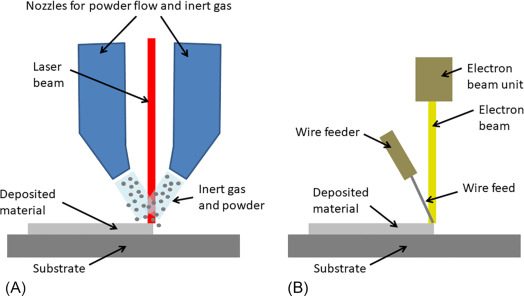
\includegraphics{lmd_1}
\ccaption{Aufbau zweier LMD-Konzepte}{\url{https://ars.els-cdn.com/content/image/3-s2.0-B9780081026632000022-f02-04-9780081026632.jpg}}
\label{img:lmd_1}	
	\end{center}
\end{figure}
Abb. \ref{img:lmd_1} zeigt die beiden wichtigisten Verfahren dieser Übergruppe: (a) \it{Laser-DED} \& (b) \it{Electron-Beam-DED}.
Bei (a) wird das Pulver durch die Düse in den Laser eingestrahlt, welcher es dann auf das darunterliegende Substrat aufträgt als geschmolzene Schweißraupe. 
Dagegen wird bei (b) mithilfe eines Elektronen-Strahls ein Draht aufgeschmolzen und in dieser Form aufgetragen. \parencite{ALL3D_1}
\subsubsection{Mehrachsen- \& Hybrid-Maschinen}
Diese Schweißraupen sind in ihren Dimensionen nicht sehr akkurat, wodurch in  industriellen Umgebungen sogenannte Mehrachsen- sowie auch Hybrid-Maschinen sehr großer Beliebtheit erfreuen. Diese verbinden die LMD-Maschine mit den subtraktiven Fertigungskapazitäten einer CNC-Fräßmaschine (\it{Computerized Numerical Control}) um die Nachbearbeitung automatisiert in den Druckprozess einzufügen. Dies ist insofern sehr vorteilhaft, dass für diese Nachbearbeitung das Werkstück nicht ausgespannt, also aus der Maschine entfernt, werden muss und dadurch keine Ungenauigkeiten durch Verschiebung des Bauteils entstehen können wie bei einem Maschinenwechsel.
Die zusätzlichen Achsen der Maschine ermöglichen es, nicht nur schichtweiße aufzutragen wie es im 3D-Druck üblich ist, sondern auch an schiefen Elementen, nachdem diese bereits gedruckt wurden oder an bereits existierenden Teilen für sogenanntes Additive Remanufacturing, also der Reperatur konventionell hergestellter Teile. \parencite{ALL3D_2}
\begin{figure}[h]
	\begin{center}
	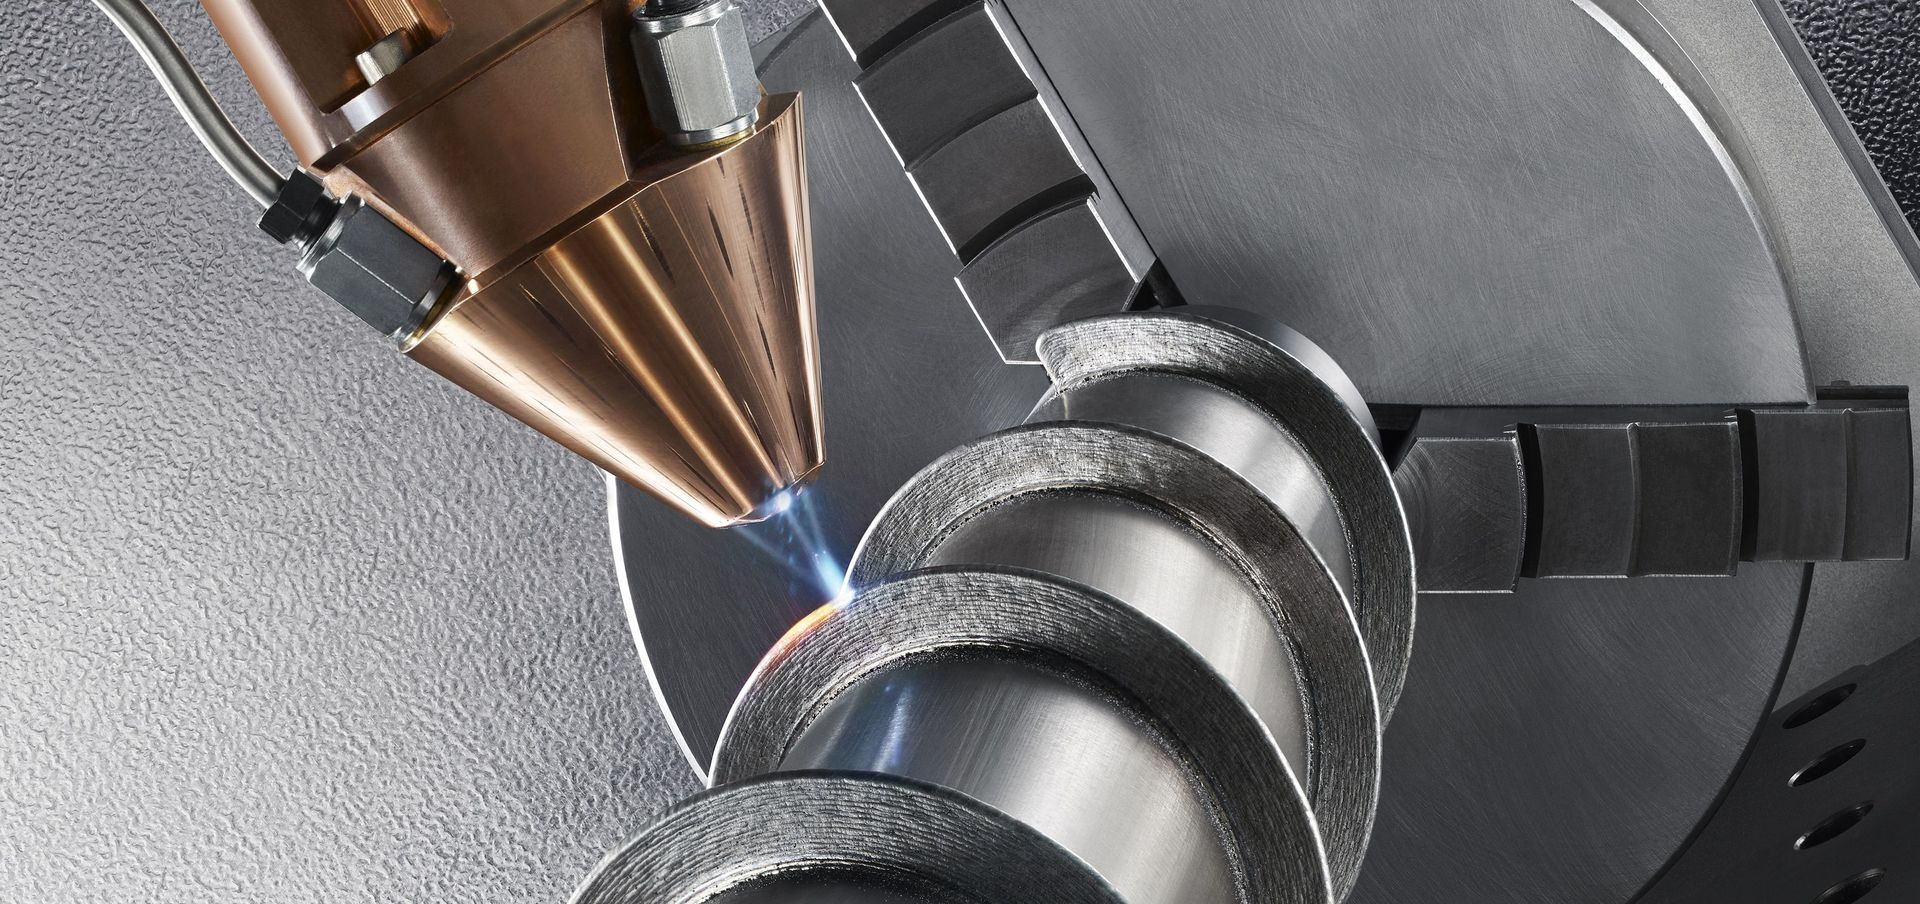
\includegraphics[width=0.8\textwidth]{lmd_part_1}	
		\ccaption{LMD Teil in Produktion auf Drehachse}{\url{https://www.trumpf.com/filestorage/TRUMPF_Master/_processed_/b/c/csm_Lasers-applications-laser-metal-deposition-process_37a1adacb9.jpg}}
		\label{img:lmd_part_1}
	\end{center}
	
\end{figure}
Abb. \ref{img:lmd_part_1} zeigt ebendies bei einem Zylinder, auf welchen auf einer Drehachse ein Gewinde neu aufgetragen wird. In der Abbildung wird der Prozess für eine neu herzustellende Gewindestange gezeigt, wobei dies auch in Zusammenarbeit mit einem 3D-Scanner auf einem beschädigte Werkstück möglich wäre. \end{document}

